\documentclass[conference]{IEEEtran}

\usepackage[noadjust]{cite}
\usepackage[pdfborder={0 0 0},bookmarks=false]{hyperref}
\usepackage[pdftex]{graphicx}
\usepackage[T1]{fontenc}
\usepackage{cleveref}
\usepackage{inconsolata}
\usepackage[listings,skins]{tcolorbox}

% \def \blindreview{} % Hide author information

\hyphenation{meta-stability}
\hyphenation{synchro-nous}
\hyphenation{veri-fication}
\hyphenation{hand-shake}

\newcommand{\mpsat}{\textsc{Mpsat}}

\title{Asynchronous Network Traversal for Computational Drug Discovery}
% lineno
\ifdefined \blindreview

	\author{
		\IEEEauthorblockN{
			\hspace{1cm}
		}
		\IEEEauthorblockA{
			\\
		}
		\\
	}

\else


	\author{
		\IEEEauthorblockN{
			Ghaith Tarawneh\textsuperscript{1},
			Alessandro de Gennaro\textsuperscript{1},
			Jonny Wray\textsuperscript{2},
			Andrey Mokhov\textsuperscript{1} and
			Alex Yakovlev\textsuperscript{1}
		}
		\IEEEauthorblockA{
			\textsuperscript{1}School of Engineering, Newcastle University, UK
			\\
			\textsuperscript{2}e-Therapeutics, UK
		}
	}


\fi


\begin{document}
\maketitle
\begin{abstract}

The availability of detailed protein-protein interaction networks or
``interactomes'' has made it possible to exploit network analysis techniques to
discover better drugs in faster and more efficient ways than ever before.
e-Therapeutics has developed a practical, in silico, approach to drug
discovery based on the construction and analysis of network representations of
disease mechanisms. Disease network construction and analysis is based on the
human interactome, a network of currently about 19K nodes linked by over 0.5M
interactions. Traversal operations on such a network are expensive and can
benefit from custom hardware acceleration. In this paper we outline two
approaches: a synchronous FPGA-based accelerator, which is very simple and
fast but limited to networks of thousands of proteins and 100s of thousands of
interactions, and an asynchronous alternative, which is more scalable and can
cope with networks comprising millions of nodes, but requires much more
sophisticated graph traversal algorithms. We present our current solution as a
challenge for the community: can you help us make it simpler?

\end{abstract}


\vspace{0.2cm}

\section{Synchronous Traversal}
\label{sec_sync}

In the first approach, we use individual flip-flops to represent network nodes
and connect these with combinational paths to form edges (\Cref{fig_mapping}).
Initially, all flip-flops have a logic low value, indicating that none of the
nodes have been visited. We~simulate network traversal by propagating a logic
high value between flip-flops, corresponding to the propagation of a
\emph{visited} state. Nodes at a distance $k$ are visited on the
$k$\textsuperscript{th} cycle, and the process completes after $D$ cycles
(where $D$ is network diameter). Here, we use OR gates to consolidate multiple
inputs (edges) and compute the next \emph{visited} state of each node.
A~global reset signal clears all flip-flops at start, after which we set one
flip-flop to begin traversal. To detect completion, we read the state of all
flip-flops and determine when all have been visited.

This approach maps very naturally to FPGAs and provides significant speedups
compared to software-based breadth-first search \cite{fdl2017}. However, many
network science applications (including computational drug discovery) use
small-world networks, characterized by their high connectivity. The abundance
of edges exhausts interconnect density on planar FPGA devices quickly, setting
an upper limit on the scale of networks that can be implemented.

\section{Challenges of Asynchrony}

Asynchronous mechanisms represent the only scalable scheme for implementing
and traversing large-scale small-world networks in hardware. This scalability
comes at the cost of extra complexity, however, since parallel (asynchronous)
traversal operations across the network are not synchronized to a common
reference and may proceed in random order.

To illustrate why asynchronous network traversal is more challenging, we will
refer to the network in \Cref{fig_async}. Here, we assume that network nodes
communicate their \emph{visited} state by exchanging asynchronous messages,
and that message delivery can occur in any order. Now, consider the problem of
determining the minimum distance between nodes $A$ and $B$. We can do this by
sending messages containing a~distance attribute $d$ between nodes, starting
with $A$, and incrementing this on each hop. Since message delivery can occur
in any order, it is possible that the chain of messages $A \rightarrow D
\rightarrow E \rightarrow B$ is delivered before $A \rightarrow B$. If so,
node $B$ will update its distance to $A$ twice, and possibly more if more
paths between $A$ and $B$ exist in a larger network. The question is: how does
$B$ determine when there are no further updates?

The example above highlights one problem that emerges due to asynchrony:
completion detection. Due to the lack of global state visibility, completion
detection is not as straightforward compared to the synchronous solution in
\Cref{sec_sync}. How can we perform asynchronous network traversal then? One
way is to implement a softer form of local synchronization between neighboring
nodes. We discuss one way to do this below.

% fig_mapping

\begin{figure}[!t]
\begin{center}

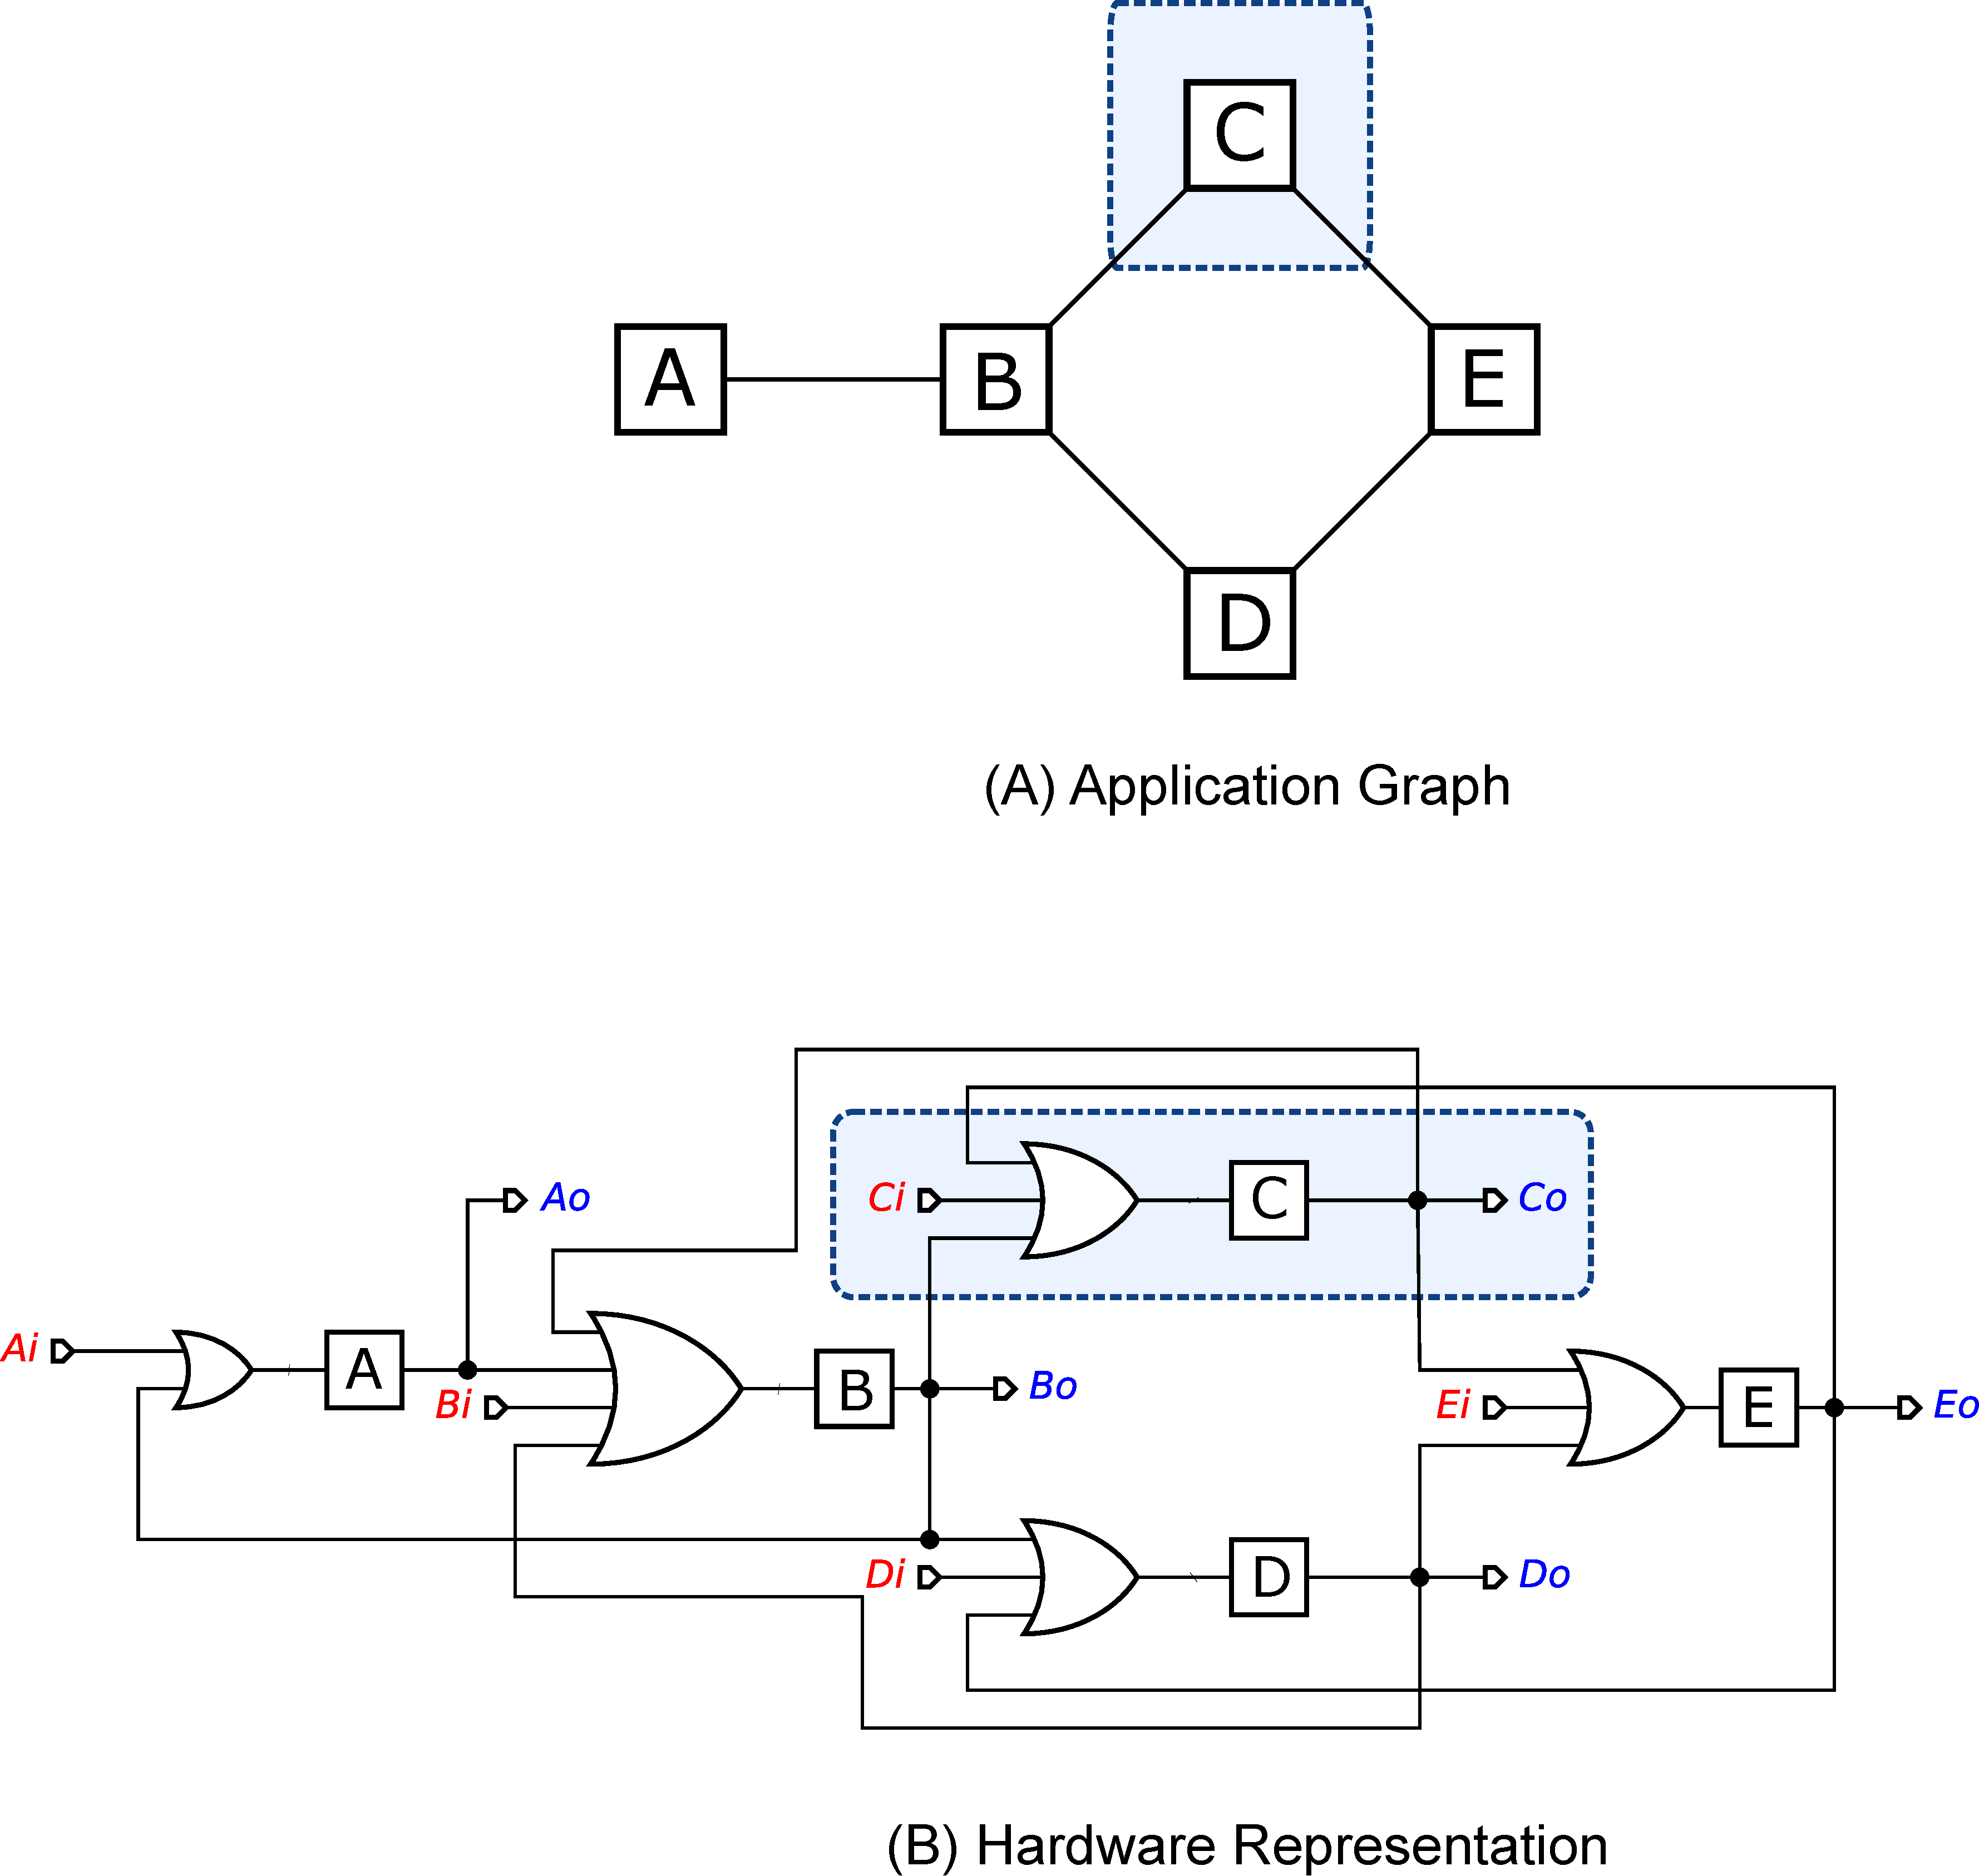
\includegraphics[width=8.8cm]{figures/fig_mapping}

\caption{
Mapping a network to hardware. Nodes are implemented as flip-flops, and edges as combinational paths.
Traversal is performed by propagating a logic high status between flip-flops, starting from a root node,
and completion is detected by monitoring the status of all nodes.
}

\label{fig_mapping}
\end{center}

\end{figure}


\section{Asynchronous Traversal}
\label{sec_async}

The proposed algorithm is from \cite{lynch1996distributed} and relies on
traversing the network multiple times with increasing depth. Each round
consists of a forward propagation of \emph{req} messages, starting from a root
node. Messages contain a hoplimit integer $h$ which is decremented on each
jump. When $h$ reaches zero, the node sends back an \emph{ack} message which
is then collated with others and funneled back to the root node. The round is
complete when the root receives \emph{ack} messages from all its neighbors.
The root then starts the next round by sending \emph{req} messages to its
neighbors, this time with an incremented hoplimit.

In the above approach, we enforce some notion of ordering because traversal
operations across the network are guaranteed to belong to the same round. We
are therefore able to detect the termination of computations at network
extremities and synchronize this back to the root. We can sum the number of
discovered nodes and relay this back via \emph{ack} messages. This provides a
method to detect completion: we terminate the algorithm after a round has been
completed and no new nodes were discovered.

\section{Future Work}

Network traversal presents an interesting problem where the conventional
benefits of asynchrony appear to come at the cost of algorithmic complexity.
Massively-parallel architectures attempting to solve such problems must rely
on asynchronous communication mechanisms for device scalability purposes
\cite{parco2017}, but may have to resort to softer forms of synchronization
for algorithmic reasons. Is this trade-off an intrinsic feature of problems
such as network traversal? If so, are there other (asynchronous) solutions
that are more optimal that one proposed \Cref{sec_async}.

\newpage

% fig_async

\begin{figure}[!t]
\begin{center}

\vspace{2.3cm}

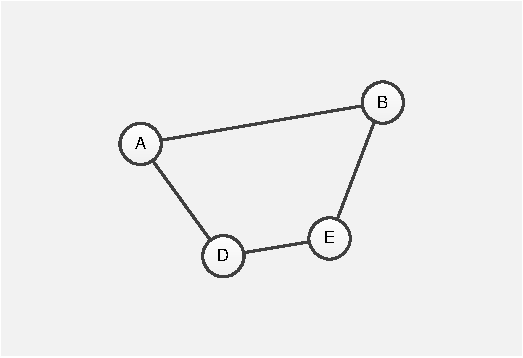
\includegraphics[width=8.8cm]{figures/fig_async}

\caption{An example to demonstrate the challenge with asynchronous network
traversal. How do we determine the minimum distance between nodes $A$ and $B$
if nodes communicate with their neighbours using asynchronous mechanisms and
the ordering of operations cannot be constrained?}

\label{fig_async}
\end{center}

\end{figure}


\section*{Acknowledgments}

This work was supported by EPSRC grant EP/N031768/1 (project POETS).

\bibliographystyle{IEEEtran}
\bibliography{bibliography}

\end{document}
